\section{Feature Dynamic}
\label{sec:dynamic}

We defined the notion of latent features previously, where features is related to the membership of nodes in latent space.  The question that we ask here, is how the total number of latent features -- its dimension -- evolve with the size of the network ie its number of vertices.

%Hence one can have theintuition that if links are mostly created in a set of class (inner or outer), the shortest path between two random nodes is``proportional'' to the number of step needed to go through all classes $K$.

The dimension of the features in the ILFM is given through the Indian Buffet Process. Though, in its metaphor, each new customers $i$ draws Poisson$(\frac{\alpha}{i})$ new dishes. Thus the expectation of the dimension of the features is:

\begin{align*}
\E[K|\alpha, N] &=  \sum_{i=1}^N \frac{\alpha}{i} = \alpha H_n \\
&= \alpha(\log(n) + \gamma +O(1/N) ) \qquad  \text{for} \quad N >> 0
\end{align*}
Where $\gamma$ is the Euler-Mascheroni constant.\\

Similarly, in a case of IMMSB, the dimension of the classes is potentially infinite and evolves with the data through an Hierarchical Dirichlet Process (HDP) prior.

In the HDP, we have two step DP that form a so called Chinese Restaurant Franchise (CRF) where each restaurant has an infinite capacity, and in its metaphor one has:
\begin{itemize}
\item The CRF has a shared menu constituted of dishes that symbolize the classes.
\item the number of table in each restaurant, where restaurant symbolically correspond to nodes and tables represent a couple of classes $(k,k')$ where a node generate some links (and non links) with other nodes. 
\item the total number of dishes in the franchise, where each table is associated to a couple of dishes, (where dishes represent the classes).
\end{itemize}

By definition of a \(DP(\alpha)\), we know that for each new draw given
\(i\) previous draws, the probability to generate a new group is equal
to \(\frac{\alpha}{\alpha +i-1}\) independently of the number of previous
component created. Moreover in the CRF, each table is drawn from a DP while the classes for each tables are drawn from one another DP (shared in all the franchise). Thus we can express the expectation of the number of tables ($\E[T|N, \alpha_0]$) and classes ($\E[K|T, \gamma]$). We start by the first quantity, for an undirected graph of size $N >> 0$:

\begin{align*}
&\E[T|N, \alpha_0] = \sum_{j=1}^N\sum_{i=1}^{2N} \frac{\alpha_0}{\alpha_0 +i-1} \\
& \alpha_0 N (\Psi(\alpha_0+2N) - \Psi(\alpha_0))
\end{align*}
Given the properties of the $\Psi$ function, we the asymptotic behavior of $\E[T|N]$ is :

\begin{equation*} \label{eq:e_t}
\E[T|N, \alpha_0] \sim \alpha_0 N \log(\frac{2N}{\alpha_0}) \qquad \text{if} \quad N >> \alpha_0 >> 0
\end{equation*}

Similarly, for the expectation of the dimension of the classes, we have:

\begin{equation*}
\E[K|T, \gamma] = \sum_{i=1}^{T} \frac{\gamma}{\gamma +i-1} = \gamma (\Psi(\gamma+T) - \Psi(\gamma))
\end{equation*}

One can remark, from equation \eqref{eq:e_t}, that $\lim_{N\to\infty} \E[T|N] \to  \infty$. Thus the expected limit for the number of cluster by chaining the two DP is:

\begin{equation*}
\E[K] = \gamma \log(\frac{\alpha_0 N}{\gamma}\log(\frac{2N}{\alpha_0} )) \qquad \text{if} \quad N >> \gamma>>0
\end{equation*}

We conclude that the latent features grow logarithmically with the number of nodes.

We show the empirical evolution of the dimension of classes generated by the HDP that we reported in figure \ref{fig:gen_dyn}. 

\begin{figure}[h]
	\centering
	
	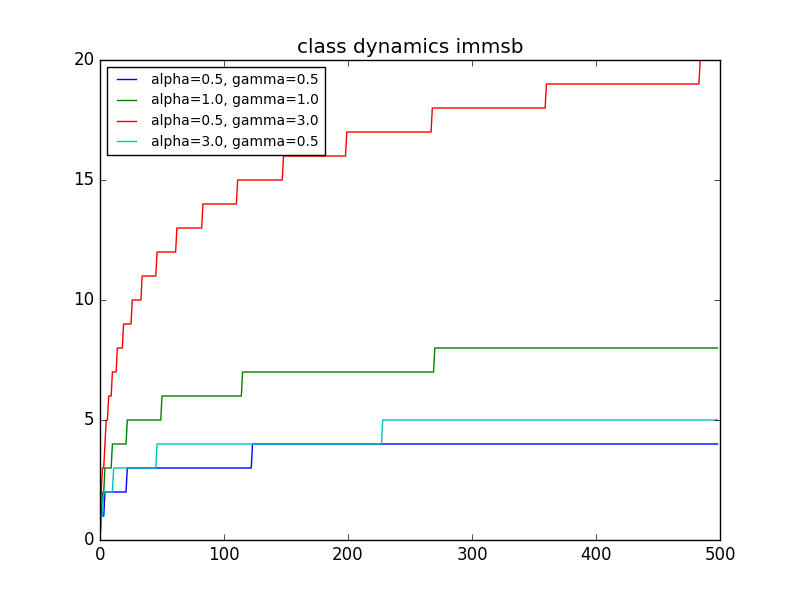
\includegraphics[scale=0.4]{img/class_dynamics}
	%	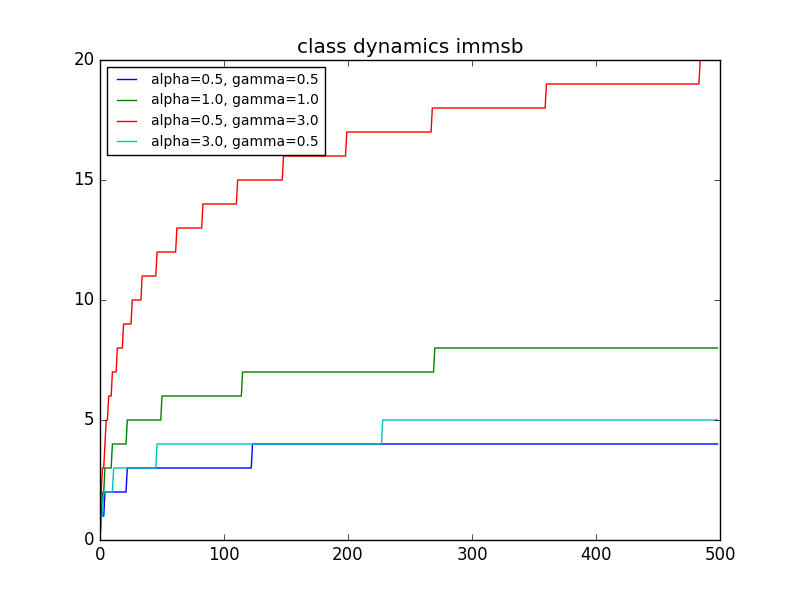
\includegraphics[width=3.2cm, height=3.7cm]{img/class_dynamics}

	\caption{Each curve correspond to a different setting of hyperparameters for IMMSB. For each X-axis correspond the nomber of nodes, for which we generated a networks. The Y-axis is the number of latent features to which HDP converged. Those figure illustrate the logarithm shape of the evolution of number of feature $K$ with the number of nodes $N$ in the networks.}
	\label{fig:gen_dyn}
\end{figure}

